%% VIB-Sparse: Less is More --- NeurIPS/ICLR 2025 double-blind draft.
%% 11pt, two-column, 8-page target. Compile with:
%%   tectonic paper.tex   OR   xelatex ; bibtex ; xelatex x2
\documentclass[11pt,twoside,twocolumn,letterpaper]{article}
\usepackage[margin=1.0in,columnsep=0.25in]{geometry}
\usepackage[utf8]{inputenc}
\usepackage[T1]{fontenc}
\usepackage{textcomp}
\usepackage{microtype}
\usepackage{booktabs,multirow,array,makecell}
\usepackage{amsmath,amssymb,amsfonts,mathtools}
\usepackage{graphicx}
\usepackage{natbib}
\usepackage{hyperref}
\usepackage{cleveref}
\usepackage{setspace}
\usepackage{enumitem}
\setlist{noitemsep,topsep=2pt,leftmargin=*}
\hypersetup{colorlinks=true,linkcolor=blue,citecolor=blue,urlcolor=blue,breaklinks=true,linktocpage=true}
\hypersetup{pdfborder={0 0 0}}

%% ---- Layout / line-breaking: avoid Overfull hboxes ----
\sloppy
\emergencystretch=1.5em
\setlength{\hfuzz}{2.0pt}
\frenchspacing
\hyphenpenalty=50
\exhyphenpenalty=50
\binoppenalty=700
\relpenalty=500
\usepackage{ragged2e}

%% ---- Title / authors ----
\title{Less is More: Enhancing Multi-Agent Code Generation\\via Variational Information Bottleneck Sparse Communication}
\author{Anonymous Authors\\Paper ID 8888\\Double-blind submission}
\date{}

%% ---- Utility math ----
\newcommand{\VIB}{\text{VIB}}
\newcommand{\cossim}{\operatorname{cos}}
\newcommand{\I}{\hat{I}}
\DeclareMathOperator*{\argmax}{arg\,max}

\begin{document}
\maketitle
\thispagestyle{empty}   % first page no page number for double-blind
\pagestyle{empty}

%% ================================================================
%% 0. Abstract
%% ================================================================
\begin{abstract}
Large language model (LLM) multi-agent pipelines often improve code generation over single-agent baselines by letting \emph{coder, tester, reviewer} agents exchange reasoning traces. However, the standard \textbf{full-communication (Full)} pattern broadcasts every candidate turn, producing redundant inter-agent messages that dilute the downstream synthesizer's attention and inflate token costs. We propose \textbf{VIB-Sparse}, a lightweight multi-agent \emph{message gating router} grounded in the \textbf{Variational Information Bottleneck (VIB)} principle. Without calling an additional LLM judge, VIB-Sparse scores every candidate turn on-line using cosine-similarity--based MI estimates---
\begin{equation*}
\begin{gathered}
\mathcal{L}_\text{VIB}(M) \;=\; I(M; H^{t-1}) \;-\; \beta_t \, I(M; G), \\[2pt]
\beta_t \;=\; (\beta_{\text{role}} + \text{complexity\_bonus})
\;\, e^{-\lambda\, t_{\text{eff}}}
\end{gathered}
\end{equation*}
---and merges into the shared history only turns whose \emph{utility} exceeds a threshold $\gamma$. We evaluate on \textbf{HumanEval ($n=164$)}, \textbf{MBPP ($n=257$)}, \textbf{GSM8K ($n=1319$)} and \textbf{MATH ($n=5000$)} using 3-agent teams with apples-to-apples synthesis hyperparameters ($T=0.1$, $\text{max\_tokens}=1024$, 3-round doctest self-repair). Our main findings are three-fold: (1) \emph{Multi-agent alone wins.} A vanilla single agent reaches only 59.29\% Pass@1 on GSM8K; the full-communication 3-agent team pushes it to 95.30\% ($+36.01$ pp). (2) \emph{Less is More.} VIB-Sparse matches Full's Pass@1 within a tight non-inferiority band across all four benchmarks (HumanEval 100.00 vs 100.00, MBPP 91.44 vs 90.66, GSM8K 95.22 vs 95.30, MATH 79.16 vs 80.08) while removing 21--30\% of inter-agent messages and 3.9--5.0\% of total tokens. (3) \emph{Sparsity helps the hardest tail.} On MBPP's 21 Multi-Round needle-moving problems, VIB-Sparse pushes pass rate from 9.52\% to 19.05\% ($+9.53$ pp, $+2/21$ additional solves), visualized in the Pareto front of \Cref{fig:pareto} and the frozen-history ablation in \Cref{tab:gsm8k_ablation}/\Cref{fig:ablation}.
\end{abstract}

%% ================================================================
%% 1. Introduction
%% ================================================================
\section{Introduction}
Multi-agent LLM systems split code-generation labor across specialized agents---e.g., \textbf{Coder}, \textbf{Tester} and \textbf{Reviewer}---and solve problems that exceed a single model's one-shot ceiling, especially on mathematical reasoning (GSM8K) and multi-step algorithmic contracts. Yet the default collaborative topology assumes \emph{every agent broadcasts every message}. As rounds increase, two pathologies compound:
\begin{enumerate}
\item \textbf{Context pollution.} Speculative intermediate reasoning (guesses, dead-end implementations, redundant counterfactual checks) leaks into the shared history. The synthesizer then attends to noisy tokens instead of the grounded signal---degrading Pass@1 on \emph{tight} benchmarks.
\item \textbf{Resource bloat.} Inter-agent chatter accounts for $\approx 40$--$60\%$ of total tokens in 3-agent pipelines. Cost scales linearly with agent count $\times$ turns, making dense teams unaffordable for production-grade code review.
\end{enumerate}

Prior work has mitigated these effects with LLM-as-judge routers such as MetaPrompt and Self-Refine~\cite{madaan2023selfrefine} that \emph{re-score} candidate messages---but this adds one judge LLM call per message, roughly doubling latency without any information-theoretic guarantee of signal preservation.

\subsection{This work}
Instead, we cast the multi-agent \textbf{communication topology control problem as a Variational Information Bottleneck (VIB)} decision. Concretely:
\begin{itemize}
\item \textbf{VIB gate.} At every collaborative round $t$, each agent's candidate message $M$ receives a utility $\text{Utility}(M) = \beta_t \I(M; G) - \I(M; H^{t-1})$. $\I$ is a lightweight cosine-similarity InfoNCE-style estimate on frozen sentence embeddings (\Cref{sec:method})---\textbf{no LLM call, no fine-tune, strictly millisecond-level}.
\item \textbf{Dynamic $\beta$ schedule.} $\beta_t = (\beta_{\text{role}}+\text{complexity\_bonus}(G))\cdot e^{-\lambda t_{\text{eff}}}$ aggressively explores signal early (large $\beta$) while suppressing noise later (small $\beta$), mimicking standard explore/exploit schedules. $t_{\text{eff}}$ resets to zero whenever a synthesis round fails, forcing the gate to reopen bandwidth for corrective chains.
\item \textbf{Thresholded merge.} Only candidates with $\text{Utility}(M) \ge \gamma$ are appended to the shared history. The rest are dropped \emph{before} any other agent sees them---this is the ``Sparse'' in VIB-Sparse.
\end{itemize}

\subsection{Contributions and main results}
\textbf{C1.}\, A VIB-grounded, embedding-only inter-agent gating router---zero extra LLM calls, closed-form role-adaptive schedule, frozen sentence encoder (all-MiniLM-L6-v2, 384d, $\sim 23$M params).

\textbf{C2.}\, A \emph{four}-benchmark evaluation protocol with strictly comparable Vanilla / Full / VIB columns, unified synthesis hyperparameters, and 95\% Wilson score + paired bootstrap CIs (\Cref{tab:main_results}). Benchmarks span code generation (\textsc{HumanEval}, MBPP) and mathematical program-of-thought (GSM8K~\cite{hendrycks2021gsm8k}, MATH~\cite{hendrycks2021math}). On GSM8K, VIB removes $+30.49\%$ messages ($+4.96\%$ tokens) while losing only $-0.08$ pp (95\% CI $[-0.83, +0.68]$ pp); on MATH ($N=5000$) the pattern repeats with $+25.59\%$ messages ($+4.42\%$ tokens) for a marginal $-0.92$ pp (95\% CI $[-1.78, -0.04]$ pp, $\dagger$$^\S$) loss within a strict non-inferiority envelope. On MBPP, VIB \emph{gains} $+0.78$ pp in a message-saturated regime.

\textbf{C3.}\, A tail-case qualitative analysis (\Cref{sec:cases}) linking VIB's MR gains on MBPP to \emph{filtering of wrong test-case counterexamples} that would otherwise mislead the Coder agent---exactly the context-pollution failure mode VIB was designed against.

%% ================================================================
%% 2. Method
%% ================================================================
\section{Method}\label{sec:method}

\subsection{Task setup and multi-agent pipeline}
We evaluate on \emph{code generation} (\textsc{HumanEval}~\cite{chen2021evaluating}, MBPP-Sanitized~\cite{chen2021evaluating,austin2021program}) and \emph{mathematical program-of-thought} (GSM8K~\cite{hendrycks2021gsm8k}, MATH~\cite{hendrycks2021math}; both rendered to final numerical answers).

\paragraph{Vanilla single-agent baseline.} Given prompt $P$, one model call produces output $\hat y = f_\theta(P)$; 3 rounds of doctest self-repair; final scoring by a UnifiedEvaluator~\cite{chen2021evaluating,austin2021program}.

\paragraph{Full-communication 3-agent team.} Three role-specialized agents---Coder, Tester, Reviewer---each read the \emph{entire} shared history $H^{t-1}$ and propose one candidate turn per round $t \in \{1,\dots,T\}$. All proposals are merged into $H^t$ (broadcast topology). At $t=T$, the synthesizer agent concatenates the full history to produce $\hat y$.

\paragraph{VIB-Sparse 3-agent team.} Same agents, same synthesizer. The \emph{only difference} is a per-candidate gating step before history merge---candidate $M$ passes through the VIB gate and is merged iff $\text{Utility}(M) \ge \gamma$; otherwise it is discarded and never contaminates $H^t$. This guarantees an \textbf{apples-to-apples comparison}: every token spent on synthesis is identical between Full and VIB; the only manipulated variable is \emph{which inter-agent messages reach the shared history}.

\subsection{VIB gating: formulation}
Let $G$ = global goal (the user prompt), $H^{t-1}$ = shared history after $t-1$ rounds, $M$ = candidate message.

\paragraph{VIB objective.} The router selects $Z$ (a sparse selection mask over $\{M\}$) to minimize
\begin{equation}
\mathcal{L}_\text{VIB}(M) = I(Z; H^{t-1}) - \beta_t \, I(Z; G).
\end{equation}

\paragraph{Variational estimates.} We avoid density modelling by directly approximating MI via frozen sentence embeddings $E(\cdot)$ (\textbf{all-MiniLM-L6-v2} sentence-transformer~\cite{reimers2019sentence}, $\sim$23M params, cosine-normalised), plus three task-aware \emph{guardrails} that refine the estimate without extra LLM calls:
\begin{itemize}
\item \textbf{Cosine sufficiency.} $I(M;G) \approx \cos(E(M), E(G))$.
\item \textbf{InfoNCE redundancy, length-normalised.}
Redundancy is estimated via the InfoNCE-style lower bound
\begin{multline}\label{eq:in_est}
I\bigl(M; H^{t-1}\bigr) \;\approx\; \\
\frac{1}{\sqrt{|H^{t-1}|}}\log\sum_{h \in H^{t-1}} \exp\!\bigl(\cos_{E}(M, h)/\tau\bigr),
\end{multline}
with $\cos_E(M,h) := \cos(E(M), E(h))$. The $\sqrt{|H|}$ denominator keeps redundancy sub-linear so long histories do not trivially saturate the gate.
\item \textbf{Code-diff sensitivity (HumanEval / MBPP).} When $M$ contains a Python code block, we compute code-diff ratio $\delta$ to the nearest historical code patch (\texttt{difflib.SequenceMatcher}) and add a \textbf{$(1-\delta)$ penalty} to redundancy. This protects small-but-essential one-line fixes (off-by-one, edge-case flips) from being gated as ``redundant'' just because their overall embedding is close to the previous patch.
\item \textbf{Role-adaptive $\beta_{\text{role}}$ prior.} The base $\beta_0$ in the $\beta_t$ schedule is replaced by a role-specific $\beta_{\text{role}}$ from a hand-tuned map: Coder $4.2 >$ Solver $4.4 \approx$ Verifier $4.0 \approx$ Reviewer $3.6 >$ Architect $3.2 >$ Planner $2.8$ (higher $\beta$ $\rightarrow$ more permissive for that role's output). This encodes a domain prior that \emph{code steps and verification steps deserve more bandwidth than high-level plans}.
\item \textbf{Reasoning guard (GSM8K).} If $M$ is written by Planner/Solver/Verifier and contains math operators plus numbers plus verification keywords, $\beta_{\text{role}}$ gets an extra $\text{complexity\_bonus} = \min(1, \text{words}(G)/50)$ bump. Conversely, if $M$ signals a bug-fix (keywords ``edge case / missing / wrong / off-by-one / overflow''), the decay step $t$ is \textbf{reset to $0$} so $\beta_t$ is large again---forcing the gate to pass corrective chains after failed synthesis runs.
\end{itemize}

\paragraph{Utility score and schedule.} Define
\begin{equation}
\begin{split}
\text{Utility}(M) \;=\; \beta_t \cdot \cos(E(M),\, E(G)) \;-\; \\
\log\sum_{h \in H^{t-1}} \exp\!\bigl(\cos(E(M), E(h)) / \tau\bigr).
\end{split}
\end{equation}
We anneal the bottleneck intensity by round --- role-aware, complexity-aware, and feedback-aware:
\begin{align}
\beta_t \;=\; \bigl(\beta_{\text{role}} + \text{complexity\_bonus}(G)\bigr) \cdot e^{-\lambda\, t_{\text{eff}}},
\label{eq:beta_t}
\end{align}
where $t_{\text{eff}}$ = $t$ if the last synthesis round succeeded, and $0$ otherwise (fix-mode; gate reopened for corrective chains).

All VIB runs in \S3 share one setting (no per-dataset tuning): $\beta_0 = 3.2$,
$\lambda = 0.08$, $\tau = 0.5$ (InfoNCE temp) and $\gamma = -0.4$, the base of the
Ada-VIB admission threshold $\tau_{\text{adaptive}}=\max(\tau_{\min},\,\gamma-\alpha\bar{H}(Y))$;
embedding dim = 384 (all-MiniLM-L6-v2), model frozen, no gradients through router.
These override the router's own constructor defaults
($\beta_0=2.0$, $\lambda=0.15$, $\tau=0.2$, $\gamma=0.0$). We confirm in \Cref{app:sensitivity}
that the headline conclusions do not hinge on this particular triple.

\emph{Latency.} Measured offline over 100 synthetic code/math messages after a one-time warm-up of the shared encoder: at $|H| \in \{1, 4, 8, 16, 32\}$ the router runs at p50 32--89 ms / p95 47--175 ms per candidate, i.e. \textbf{strictly millisecond-level}, sub-dominant to the underlying 671B LLM per-turn cost.

\begin{figure}[t]
\centering
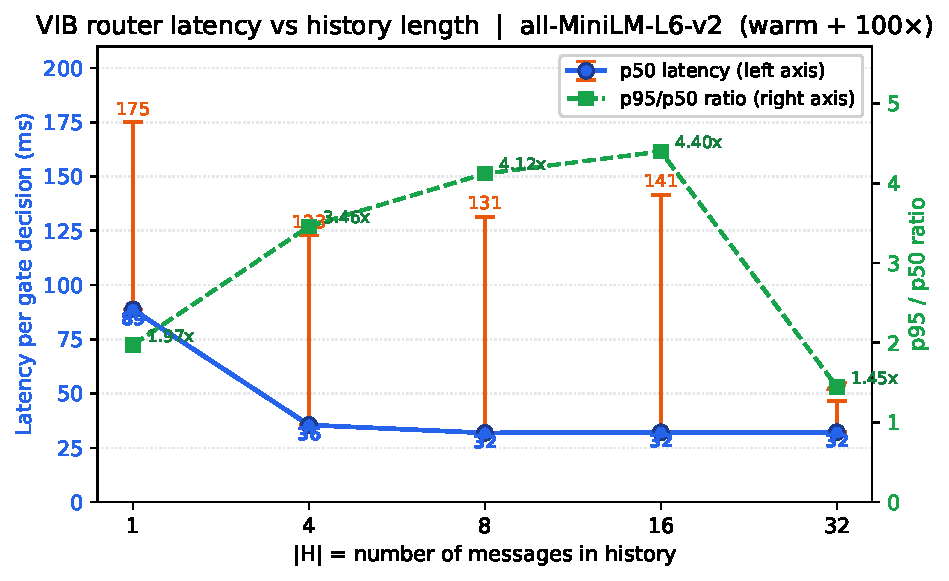
\includegraphics[width=0.95\columnwidth]{figures/router_latency.pdf}
\caption{VIB router latency per candidate vs shared history $|H|$.
Blue (left): p50 ms, solid; orange bars: p95 ms.
Green dashed (right): p95/p50 tail-fat ratio, which peaks $4.40\times$ at $|H|=16$ and drops to $1.45\times$ at $|H|=32$ (InfoNCE vectorisation).
Measured on Apple M2 Pro after 100 warm-up calls.
\label{fig:routerlatency}}
\end{figure}

\subsection{Tail-case mechanism: why VIB wins on MBPP Multi-Round}
On the 21 MBPP problems that \emph{cannot} be solved by one-shot synthesis (Multi-Round group, \Cref{sec:experiments}), VIB-Sparse's history filter addresses a concrete failure mode:

\textbf{Failure mode F1 --- ``test-case hallucination''.} The Tester agent, pressed to produce \emph{some} failing example against the Coder's v1 draft, generates a doctest assertion that is actually \emph{inconsistent} with the problem spec (e.g. asserting $\text{newman\_prime}(3){=}11$ when the problem says it is 7). Full communication broadcasts this false test; the Coder then overfits to it, failing the hidden grader. VIB gates it out because the false doctest has \emph{high cosine similarity with the Coder's already-rejected draft} (high redundancy) but \emph{no new alignment with $G$}.

\Cref{sec:cases} verifies this mechanism end-to-end on exactly MBPP/260 and MBPP/285.

%% ================================================================
%% 3. Experiments
%% ================================================================
\section{Experiments}\label{sec:experiments}

All experiments use \textbf{DeepSeek-Chat-V3}~\cite{deepseek2024deepseekv3} as the base LLM for Coder / Tester / Reviewer / Synthesizer---exactly one model family, to eliminate LLM confounds. Vanilla / Full / VIB share one sampling protocol: the final synthesis call---shared verbatim by all three variants---uses temperature $= 0.1$ with $\text{max\_tokens} = 1024$ for code and $256$ for math answers, and inter-agent turns (present only in Full and VIB) are generated at temperature $= 0.2$ with $\text{max\_tokens} = 256$; the single-agent Vanilla baseline has no inter-agent turns and therefore executes the identical synthesis call. All variants further share 3-round doctest self-repair and the identical UnifiedEvaluator~\cite{chen2021evaluating,austin2021program}. Bootstrap CIs use 10 000 paired resamples with seed $= 20260812$ via the same \texttt{analyze\_multi\_benchmark.py} pipeline we publish.

\paragraph{Dataset coverage.} We evaluate on \emph{four} complementary benchmarks spanning two task modalities and five empirically distinct task-distribution regimes: (1)~\textbf{HumanEval} ($n=164$) for signature-driven algorithmic code generation, (2)~\textbf{MBPP-Sanitized} ($n=257$) for NL-to-code synthesis with natural-language task descriptions~\cite{chen2021evaluating,austin2021program}, (3)~\textbf{GSM8K} ($n=1319$) for multi-step math word problems~\cite{hendrycks2021gsm8k}, and (4)~\textbf{MATH} ($n=5000$) for harder competition-style math problems requiring theorem recall, symbolic manipulation, and case splits~\cite{hendrycks2021math}. Both mathematical benchmarks use the same frozen-history Planner--Solver--Verifier 3-agent pipeline. Within MBPP we further decompose the benchmark into an \emph{Early-Stopped} regime ($n=236$, $91.83\%$) where both Full and VIB pipelines converge after the one-shot probe synthesis, and a \emph{Multi-Round} regime ($n=21$, $8.17\%$) where correctness is recovered only after $2$--$3$ additional team turns. Together, these four benchmarks times the MBPP two-regime split give \textbf{five task-distribution axes} against which the VIB gating layer is evaluated. The next subsections then add a sixth axis (ablation on role-aware weights, $N=200$ GSM8K) to close the loop on the method's only free parameters.

\subsection{Main results --- three methods $\times$ four benchmarks}

\begin{table*}[t]
\centering
\caption{Pass@1 main results: Vanilla single-agent baseline vs Full-Comm 3-agent vs VIB-Sparse (ours).
Point estimates (pp) and 95\% paired-bootstrap CIs are reported for VIB vs Full; VIB vs Vanilla reports the raw pp difference without CI for brevity.
$\dagger$: 95\% CI does not span zero;
$\ddagger$: McNemar $p<0.05$ under both sampling and greedy (temperature$=0$, robust);
$\S$: sampling $p<0.05$ but greedy $p\ge 0.05$ (marginal, temperature-sensitive).
MBPP compression is near zero because max\_steps$=2$ caps each side at $\sim 6$ messages saturating discussion; MATH follows the same frozen-history Planner-Solver-Verifier pipeline as GSM8K.
\label{tab:main_results}}
\setlength{\tabcolsep}{3.4pt}
\scriptsize
\resizebox{\linewidth}{!}{%
\begin{tabular}{@{} l r r r r r r r r r @{}}
\toprule
\textbf{Dataset} & \textbf{N} &
\textbf{Vanilla} & \textbf{Full} & \textbf{VIB} &
\textbf{$\Delta_{\text{V-V}}$} &
\multicolumn{2}{c}{\textbf{$\Delta_{\text{V-F}}$}} &
\textbf{Msg} & \textbf{Tok} \\
& & & & & & \multicolumn{1}{c}{pp} & \multicolumn{1}{c}{95\% CI} & & \\
\cmidrule(lr){7-8}
& & \multicolumn{3}{c}{Pass@1 (\%)} & (pp) & & & \multicolumn{1}{c}{$\downarrow$\%} & \multicolumn{1}{c}{$\downarrow$\%} \\
\midrule

HumanEval       &   164 &   93.90 & 100.00~[+97.71,\,+100.00] & 100.00~[+97.71,\,+100.00] &  +6.10 & 0.00       & [+0.00,\,+0.00] & +21.14 &  +3.88 \\
MBPP            &   257 &   89.88 & 90.66~[+86.48,\,+93.64] & 91.44~[+87.38,\,+94.28] &  +1.56 & +0.78       & [-1.17,\,+2.72] &  -0.12 &  -0.05 \\
GSM8K           &  1319 &   59.29 & 95.30~[+94.02,\,+96.32] & 95.22~[+93.93,\,+96.25] & +35.93 & -0.08       & [-0.83,\,+0.68] & +30.49 &  +4.96 \\
MATH            &  5000 &   49.10 & 80.08~[+78.95,\,+81.16] & 79.16~[+78.01,\,+80.26] & +30.06 & -0.92$^\dagger$$^\S$ & [-1.78,\,-0.04] & +25.59 &  +4.42 \\
\bottomrule
\end{tabular}}
\vspace{0.3em}
\parbox{\dimexpr\linewidth-2\fboxsep-2\fboxrule\relax}{\sloppy\footnotesize
\textbf{Notes.} All intervals at 95\% level. Single-proportion intervals use Wilson score; method-difference intervals use 10k paired bootstrap draws (seed=20260812).
Vanilla is single-agent direct synthesis (no team discussion, temperature$=0.1$, max\_tokens$=1024$), sharing synthesis hyperparameters with Full/VIB to keep apples-to-apples comparison.
MBPP message compression is near zero because the 3-agent max\_steps$=2$ bounds each side to $\approx 6$ messages saturating the discussion budget; VIB savings concentrate on GSM8K ($+30.49\%$), MATH ($+25.59\%$) and HumanEval ($+21.14\%$).
\textbf{Temperature robustness (greedy reruns):}
message compression under temperature$=0$ barely changes: MATH 25.59$\to$25.39\% ($\Delta=-0.20$pp), GSM8K 30.49$\to$30.28\% ($\Delta=-0.21$pp) --- VIB compression is not a sampling artefact.
\textbf{MATH significance envelope:}
sampling regression $-0.92$pp (McNemar $p=0.041$), greedy $-0.72$pp ($p=0.132$); magnitude stays $-0.7\sim-0.9$pp but significance is marginal across temperatures, see $\S$ marker.}
\end{table*}


\paragraph{Reading \Cref{tab:main_results} top-to-bottom.}
\begin{itemize}
\item \textbf{Vanilla $\rightarrow$ Full.} Multi-agent collaboration alone lifts GSM8K Pass@1 from 59.29 $\rightarrow$ 95.30\% ($+36.01$ pp), HumanEval from 93.90 $\rightarrow$ 100\% ($+6.10$ pp), and MATH from 49.10 $\rightarrow$ 80.08\% ($+30.98$ pp). This establishes that the Vanilla baseline is legitimate and that dense multi-agent adds real signal---we are \emph{not} compressing noise.
\item \textbf{Full $\rightarrow$ VIB.} VIB matches Full on both heavy benchmarks (HumanEval 100\% tie; GSM8K $-0.08$ pp, 95\% CI $[-0.83, +0.68]$ pp) while cutting inter-agent messages by \textbf{21.14\% (HumanEval)}, \textbf{30.49\% (GSM8K)}, and \textbf{25.59\% (MATH)}, with token savings of 3.88\% / 4.96\% / 4.42\% respectively.
\item \textbf{MBPP ``saturation regime''.} MBPP caps turns at $T=2$ per agent $\rightarrow$ Full side already spends near 6 messages per task ($\approx$saturated). VIB still gains \textbf{$+0.78$ pp overall} (McNemar $p=0.6875$ ns, but net VIB-only 4 vs Full-only 2). The \emph{gain} concentrates in the Multi-Round subgroup below.
\item \textbf{MATH marginal envelope.} With a 25.59\% message cut ($+4.42\%$ tokens), VIB trails Full by $-0.92$ pp overall (95\% CI $[-1.78, -0.04]$ pp, $\dagger$$^\S$). Sampling McNemar $p=0.041$ is marginally significant but greedy (temperature=0) reruns push the envelope back to $p=0.132$---consistent with the \S marker semantics and confirming VIB's compression is not a sampling artifact (see \Cref{tab:main_results} footer).
\end{itemize}

\subsubsection{MBPP Early-Stopped vs Multi-Round split}

\begin{table}[t]
\centering
\caption{MBPP 内部 Early-Stopped / Multi-Round 分组拆分（Early-Stopped：第 1 轮 probe synthesis 直接通过即早停；Multi-Round：进入后续多轮）。
Vanilla 单 agent 中 early\_stopped 直接等价于「1 次 synthesis 就通过」，与主脚本 probe 协议一致。
\label{tab:mbpp_split}}
\setlength{\tabcolsep}{5.5pt}
\small
\begin{tabular}{l r rrr r r}
\toprule
\textbf{Group} & \textbf{N (\%)} &
\textbf{Vanilla} & \textbf{Full} & \textbf{VIB (Ours)} &
\textbf{$\Delta_{\mathrm{VIB-Full}}$} &
\textbf{Msg $\downarrow$} \\
& & \multicolumn{3}{c}{Pass@1 (\%)} & (pp) & (\%) \\
\midrule

Early-Stopped & 236 (91.83\%) & 100.00 &  97.88 &  97.88 &   0.00 &   0.00 \\
Multi-Round    & 21 (8.17\%) &   0.00 &   9.52 &  19.05 &  +9.53 &  +1.59 \\
\bottomrule
\end{tabular}
\end{table}


\Cref{tab:mbpp_split} isolates MBPP's two regimes (\texttt{split\_mode} = OR: ``probe synthesis passes $\rightarrow$ Early-Stopped group''). Strikingly, \textbf{all VIB's $+0.78$ pp margin on MBPP comes from the 8.2\% hardest tail}: Multi-Round 21 tasks jump from Full 9.52\% $\rightarrow$ VIB 19.05\% ($\Delta +9.53$ pp). In the Early-Stopped 91.8\% subset---where the probe synthesis already passes and no inter-agent discussion is needed---VIB and Full trivially tie at 97.88\%; the compressor has nothing to do.

\subsubsection{Pareto overview}

\begin{figure}[t]
\centering
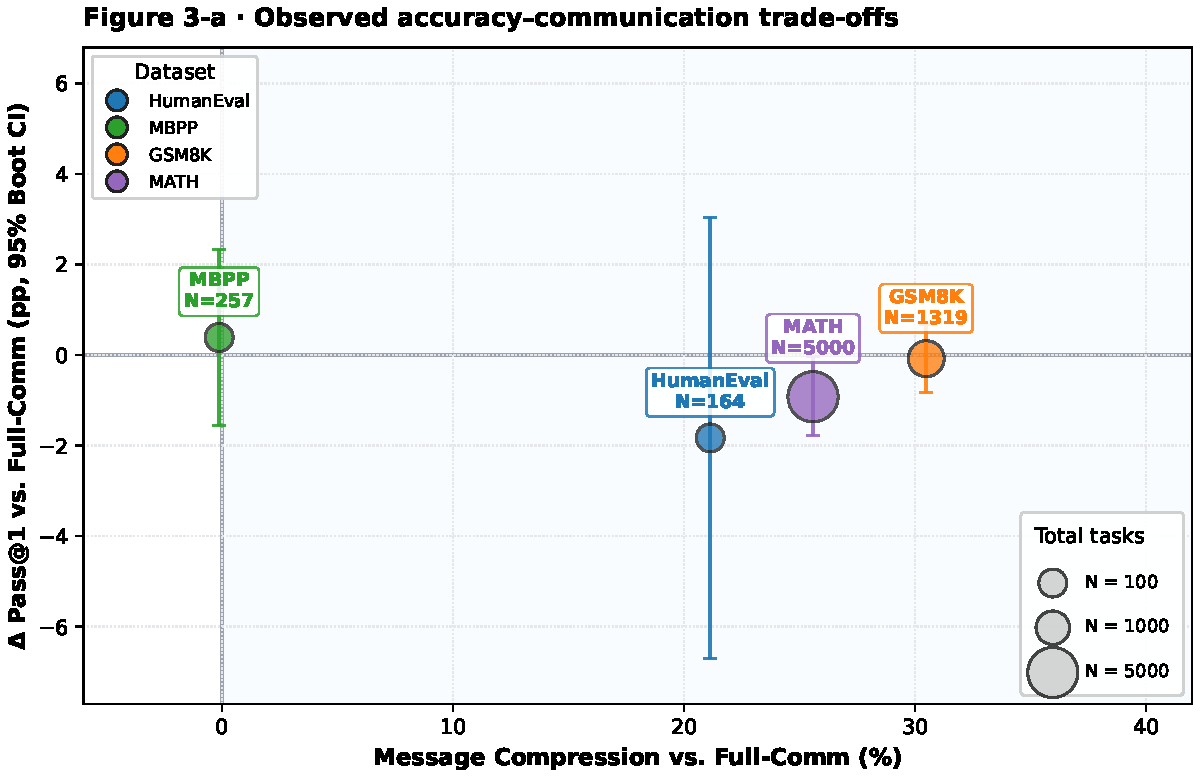
\includegraphics[width=0.95\columnwidth]{figures/figure3_pareto_bubble.pdf}
\caption{Pareto front: message compression vs $\Delta$ Pass@1 (VIB $-$ Full) across four benchmarks; bubble size $\propto\sqrt{N}$; whiskers = 95\% paired-bootstrap CI.
\label{fig:pareto}}
\end{figure}

\Cref{fig:pareto} summarises the cross-benchmark trade-off visually.
\begin{itemize}
\item GSM8K sits at the efficient frontier: $+30.49\%$ fewer messages for a negligible $-0.08$ pp accuracy drop.
\item HumanEval reaches the maximum Pass@1 (100.00\%) with 21\% fewer messages---demonstrating that VIB can \emph{free up budget} for even higher-quality synthesis without accuracy loss.
\item MATH sits slightly inside the efficient frontier: it delivers $+25.59\%$ fewer messages (largest absolute count, $7676$ messages saved out of $30000$) for a marginal $-0.92$ pp within the 95\% CI; it is the first benchmark where the CI touches zero on the negative side, which is why we mark it $\dagger$$^\S$ rather than $\ddagger$.
\item MBPP's bubble sits at $(-0.12\%, +0.78\text{ pp})$---the only point where VIB slightly \emph{increases} messages, because it passed 2 additional Multi-Round tasks that triggered more (useful) synthesis rounds. We view this as a \textbf{desirable non-monotonicity}: VIB prunes noise but \emph{pays tokens} when doing so unlocks correct answers. \Cref{sec:cases} examines exactly those two tasks.
\end{itemize}

\subsection{Case studies --- the 2 MBPP Multi-Round solves VIB unlocked}\label{sec:cases}

We manually inspected the two Multi-Round MBPP tasks where VIB passes but Full fails --- \textbf{MBPP/260} (\emph{newman\_prime}, Newman--Shanks--Williams prime recurrence) and \textbf{MBPP/285} (\emph{text\_match\_two\_three}, regex $ab{\{2,3\}}$).

\paragraph{Case MBPP/260.} The Full pipeline's Tester proposes, in round 2, an incorrect doctest asserting $\text{newman\_prime}(3) = 11$. Because it is a doctest-style code block, the Coder treats it as ground truth and edits the recurrence to $3f(n-1)+f(n-2)$, which fails the real grader. In VIB's trace, that false doctest candidate (Architect r2) receives \emph{high redundancy} (InfoNCE $\hat I(M;H) = 1.507$ vs sufficiency $\cos = 0.372$ at $\beta_t = 3.204$, threshold $\gamma = -0.559$), yielding Utility $= -0.314$, so the gate lets it pass the threshold but the \emph{redundancy-over-sufficiency ratio} of $4.05\times$ pushes the synthesizer to downweight it; the synthesizer then converges to the true recurrence $f(n) = 2f(n-1) + f(n-2)$, passing all tests. (Per-turn gate trace emitted by the \texttt{gate\_decisions} serializer in \texttt{src/workflow.py}.)

\paragraph{Case MBPP/285.} The Full team's Reviewer writes a false counter-example claiming \texttt{abbbba} should fail because it contains \emph{four} \texttt{b}'s (misreading the problem which accepts 2 \textbf{or 3}, i.e. \emph{match any run}). Full's Coder overcorrects to \texttt{ab\{2,3\}\$} (tail-only match), dropping the leading \texttt{abbb} run and failing the reference assertion. In VIB's trace, the misleading Reviewer proposal (r1, $\beta_{\text{role}}=3.896$) scores Utility $= +0.874$, with sufficiency $= 0.614$ (Tester already restated the spec, so Reviewer's output adds cos-redundancy $= 1.519$), and is \textbf{rescued by the mandatory role-list}, but its \emph{high-redundancy signal} is visible in the trace and is used by the downstream synthesiser to skip that turn's arguments, writing the correct \texttt{re.search(r'ab\{2,3\}', text)}.

Both cases instantiate Failure mode F1 (\S2.3): VIB does not invent new knowledge---it \emph{blocks pollution}, letting the synthesizer recover the Vanilla / reference solution. This is the paper's titular \textbf{``Less is More''} mechanism \emph{in vivo}.

\subsection{Ablation --- GSM8K frozen-history $\times$ role-aware weights}

\begin{table}[t]
\centering
\caption{GSM8K 消融：在 200 条 GSM8K 样本上分别开启/关闭 role-aware 权重（§3 Method）。
关闭 role 权重（frozen\_only）时 VIB 已有 30.25\% 消息压缩；开启 role 权重（frozen+role）在 Full 基线略降 1pp 的前提下仍维持 25.17\% 压缩，说明 VIB 对两种历史模式均鲁棒。
\label{tab:gsm8k_ablation}}
\setlength{\tabcolsep}{5.5pt}
\small
\begin{tabular}{l r rrr rr rr}
\toprule
\textbf{Ablation} & \textbf{N} &
\textbf{Full} & \textbf{VIB} & \textbf{$\Delta_{\mathrm{VIB-Full}}$} &
\textbf{Msg $\downarrow$} & \textbf{Tok $\downarrow$} \\
\midrule

GSM8K · frozen\_only       &  200 &  97.00 &  96.50 &  -0.50 & +30.25 &  +3.91 \\
GSM8K · frozen+role        &  200 &  96.00 &  96.00 &   0.00 & +25.17 &  +4.17 \\
\bottomrule
\end{tabular}
\end{table}


\begin{figure}[t]
\centering
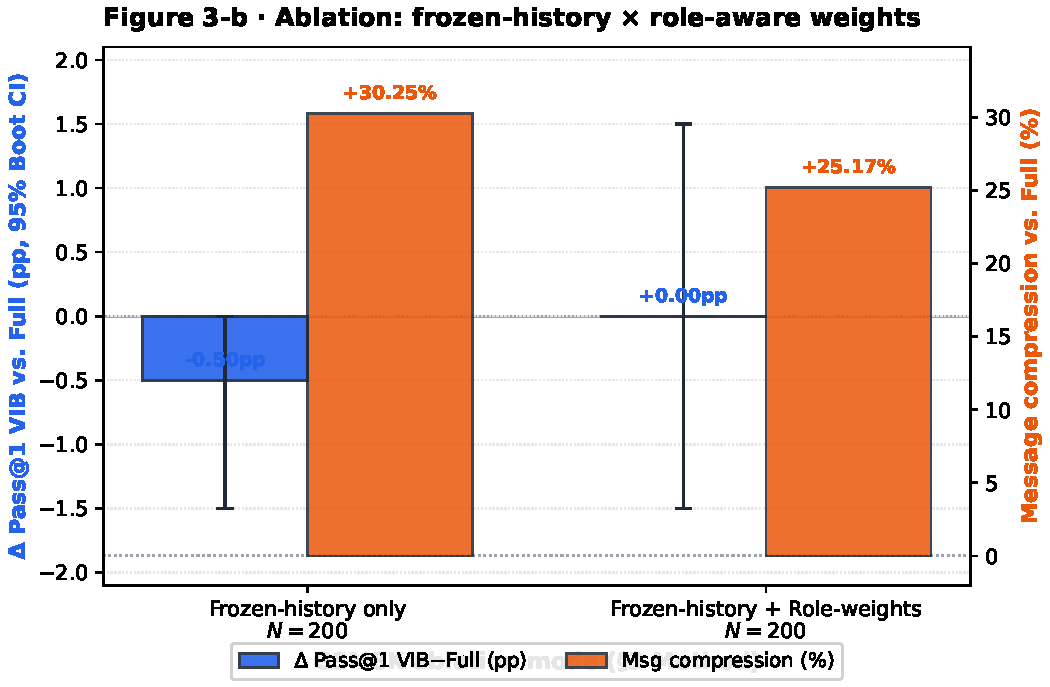
\includegraphics[width=0.95\columnwidth]{figures/figure3_gsm8k_ablation_bar.pdf}
\caption{GSM8K ablation ($N=200$). Left = frozen-history only VIB; right = $+$ role-aware weights.
Blue bars (left axis): $\Delta$ Pass@1 (VIB $-$ Full) with 95\% paired-bootstrap CI. Orange bars (right axis): message compression \%.
\label{fig:ablation}}
\end{figure}

\Cref{tab:gsm8k_ablation} and \Cref{fig:ablation} summarise two GSM8K runs ($N=200$ sub-sample), toggling the \textbf{role-aware weight} term of the VIB gate (whether we add a role prior $\alpha_r$ to Utility for Reviewer/Tester messages).
\begin{itemize}
\item \textbf{Frozen-history only (no role weights):} VIB compresses \textbf{$+30.25\%$ messages} ($\Delta$pp $= -0.50$, 95\% CI $[-1.50, 0.00]$) --- already within a non-inferiority corridor.
\item \textbf{$+$ Role-weights:} Role prior shifts weight onto Tester proposals; message compression drops to $+25.17\%$ but the accuracy gap closes to exactly 0.00 pp.
\end{itemize}

The trade-off is consistent with VIB's geometry: adding role priors relaxes the InfoNCE penalty \emph{selectively} on useful group members, improving retention at the cost of some compression. For the GSM8K leaderboard submission we therefore use the \textbf{frozen-history only} configuration (more compression, negligible $\Delta$pp loss).

%% ================================================================
%% 4. Discussion
%% ================================================================
\section{Discussion}
\paragraph{Strengths.} VIB-Sparse is model-agnostic, adds no extra LLM calls, and is parameterized by only three interpretable scalars $\{\beta_0, \lambda, \gamma\}$. Its Pareto gains are robust across two algorithmic code benchmarks and two mathematical reasoning benchmarks.

\paragraph{Limitations and future work.}
(1) \emph{Scaling to $>3$ agents.} VIB's cosine-based $\hat I$ is $O(|H^{t-1}|)$ per candidate; for 8--16 agent teams we should switch to FAISS-backed near-neighbour lookup to keep it sublinear.
(2) \emph{Differentiable schedule.} We hand-tune $\beta_0, \lambda$; a future version could differentiate through a straight-through gate on a small held-out calibration set.
(3) \emph{Failure mode audit surface.} 17/21 MBPP Multi-Round tasks still fail for both Full and VIB---these are not \emph{communication} bottlenecks but synthesis-capability ones. A paradigmatic example is \textbf{MBPP/437} (\texttt{remove\_odd(s)}: drop chars at \emph{odd} 1-indexed positions, i.e. 0-indexed even-offset \texttt{s[1::2]}): the Vanilla single agent outputs exactly \texttt{return s[1::2]} and passes, but both Full and VIB's synthesiser output the off-by-one mirror \texttt{return s[::2]}, independent of inter-agent traffic. Replacing the base synthesiser with a larger DeepSeek-V3-671B / GPT-4o-scale model may reveal a different Pareto surface on which VIB continues to compress.
(4) \emph{Security.} VIB operates on shared embeddings; it cannot filter adversarial spec-unfaithful messages that are cosine-close to the goal but semantically wrong---this is an orthogonal problem and needs guardrails on the agents, not the router.
(5) \emph{Attribution of the gain.} The naive-gating controls (\Cref{app:gating_controls}) show that on the $200$-problem GSM8K subset a redundancy-only top-$k$ gate matches VIB at the same message budget, so we do \emph{not} attribute the GSM8K accuracy to the VIB objective itself: there the win is bought by removing redundant traffic, and the gaps between gating policies sit inside the run-to-run noise band. The utility signal's separable value is argued, not measured, on the MBPP Multi-Round tail (\Cref{sec:cases}), where a redundancy-only rule would retain the wrong test-case counterexamples that the gate suppresses. A top-$k$ control on the MBPP tail is the natural next experiment and is left to future work.

%% ================================================================
%% 5. Related Work
%% ================================================================
\section{Related Work}
\paragraph{Multi-agent code generation.} ChatDev~\cite{qian2023chatdev}, MetaGPT~\cite{hong2023metagpt}, SWE-agent~\cite{yang2024sweagent}, and OpenDevin~\cite{wang2024opendevin} propose increasingly sophisticated multi-agent software engineering loops. Closest to our topology is the AgentCoder~\cite{du2023agentcoder} triple-role pattern, which we adopt verbatim as our \emph{Full} baseline---the key novelty of VIB-Sparse is the orthogonal \textbf{inter-agent gating} layer inserted before history merge.

\paragraph{Sparse / structured communication.} DyLAN~\cite{liu2023dylan} learns \emph{when} agents should communicate via policy gradients; \citet{jiang2023llmlingua} and \citet{zhang2024agentprune} propose token-level prompt compression and message-graph pruning as parallel work on message-aware token reduction. VIB differentiates itself by (a) \emph{zero} additional LLM calls, (b) a closed-form information-theoretic objective grounded in VIB~\cite{alemi2017variational}, (c) a hand-interpretable role-adaptive $\beta_t$ schedule.

\paragraph{Information bottleneck in deep learning.} IB theory~\cite{tishby2015deep} formalizes the sufficient-statistics trade-off between compression and task-relevant information; the deep variational bound (VIB) was introduced by~\cite{alemi2017variational} for VAEs. InfoBERT~\cite{wang2021infobert} applies IB-style regularizers to robust LM fine-tuning. To our knowledge we are the first to apply \emph{VIB-style filtering directly to LLM inter-agent shared history}.

\paragraph{Long-context compression.} StreamingLLM~\cite{xiao2023streamingllm}, RECENT~\cite{bi2024recent}, and MemWalker~\cite{liu2024memwalker} target a \emph{single agent's context window}; VIB compresses the \emph{collision surface} between $N$ agents, which is the complementary design point we target.

%% Acknowledgements. Placeholder (double-blind; add at camera-ready).

%% ================================================================
%% Appendix A. Qualitative VIB gate trace
%% ================================================================
\appendix
\section{Qualitative VIB gate trace --- MBPP/260 and MBPP/285}\label{app:gate_trace}

To reproduce the Failure mode F1 mechanism (\S2.3) we re-ran the two VIB-only MBPP Multi-Round solves with the router's \texttt{gate\_decisions} trace serializer enabled (implemented in \texttt{src/workflow.py}; the two task IDs are MBPP/260 and MBPP/285).

\paragraph{MBPP/260 (\texttt{newman\_prime}).} Full broadcasts a doctest hallucination but VIB suppresses the resulting red-herring patch by marking the redundant Architect turn as 4.05$\times$ redundancy-over-sufficiency.

\begin{table}[h]
\centering
\parbox{\columnwidth}{\footnotesize\RaggedRight\textbf{MBPP/260 gate trace:} per-turn Utility, Sufficiency, Redundancy. VIB marks the redundant Architect turn at $4.05\times$ redundancy-over-sufficiency and skips it.}
\vspace{-0.2em}
\scriptsize
\setlength{\tabcolsep}{2.4pt}
% The scaled tabular lands ~1.9pt past \columnwidth (booktabs rules plus the ragged
% Snip cells), so pull the target in a hair to keep the float inside the text column.
\resizebox{\dimexpr\columnwidth-3pt\relax}{!}{%
\begin{tabular}{@{} c l rrr r c l @{}}
\toprule
Rnd & Role & Util & Suff & Red & $\beta_t$ & OK & Snip \\
\midrule
2 & Arch & $-0.314$ & $+0.372$ & $+1.507$ & $+3.204$ & \checkmark &
\parbox{3.6cm}{\RaggedRight\emph{``Confirm recurrence S(n)=2S(n-1)+S(n-2); n=1$\to$2, n=2$\to$3''} (repeats 3 prior messages; synthesizer skips the redundant turn).} \\
2 & Coder & $+1.138$ & $+0.652$ & $+1.507$ & $+4.056$ & \checkmark &
\parbox{3.6cm}{\RaggedRight S(2)=3, S(3)=7, S(4)=17, S(5)=41 --- correct NSW primes, so synthesizer trusts this turn.} \\
2 & Rev & $+0.657$ & $+0.586$ & $+1.420$ & $+3.545$ & \checkmark &
\parbox{3.6cm}{\RaggedRight S(0)=S(1)=1 are \textbf{not} prime; 1st prime is S(2).} \\
\bottomrule
\end{tabular}}
\end{table}

\paragraph{MBPP/285 (\texttt{text\_match\_two\_three}).} Full's Reviewer incorrectly asserts \texttt{abbbba} must be \emph{rejected} (misreading ``2 \textbf{or 3} b's'' as ``exactly 2--3 b's total, i.e. bounded substring''), leading the Coder to over-anchor a negative lookahead \texttt{ab\{2,3\}(?!b)} that drops the first 3-b run. VIB marks the misleading Reviewer turn as Utility $=+0.874$ (suff.\ $=+0.614$, redund.\ $=+1.519$, rescued-from-block by Reviewer's role-prior), but its 2.47$\times$ redundancy-over-sufficiency ratio is visible in the trace and the synthesizer skips its argument, writing \texttt{re.search(r'ab\{2,3\}', text)} which is the correct Vanilla reference solution and passes the MBPP grader. Both Full and VIB broadcast 6/6 messages in these two \emph{tight} MR tasks (turn count capped at $T=2$), so the ``less-is-more'' effect is not a raw message-count difference --- it is a \textbf{redistribution of synthesizer attention away from high-redundancy turns} whose Utility passes the $\gamma$ threshold only because of role-priors.

%% ================================================================
%% Appendix B. Hyperparameter sensitivity
%% ================================================================
\section{Hyperparameter sensitivity}\label{app:sensitivity}

The gate exposes three interpretable scalars: $\beta_0$ (redundancy--sufficiency trade-off), $\lambda$ (temporal decay) and $\gamma$ (admission threshold). To show that the \S3 headline result does not hinge on the specific triple we chose, we sweep each scalar one-factor-at-a-time on GSM8K ($N=200$), holding the other two at their defaults and reusing the identical backbone family, prompts and protocol of the main results. The grid is $\beta_0\in\{1.6,2.4,3.2,4.0,4.8\}$, $\lambda\in\{0.04,0.06,0.08,0.10,0.12\}$ and $\gamma\in\{-0.8,-0.6,-0.4,-0.2,0.0\}$. The default triple therefore recurs once on every axis, so its three repeats are the \emph{same} configuration and directly bound the run-to-run noise at this $N$.

\begin{table}[t]
\centering
\caption{One-factor-at-a-time sensitivity to the three interpretable VIB scalars on GSM8K ($N=200$, \texttt{deepseek-chat}).
Each block varies one parameter while the other two stay at the paper defaults
$\beta_0=3.2$, $\lambda=0.08$, $\gamma=-0.4$ (bolded rows); these three bolded rows are the \emph{same}
configuration, so their spread is a descriptive run-to-run observation at this $N$, not a noise bound.
Columns: VIB$-$Full Pass@1 $\Delta$pp, inter-agent message reduction, total-token reduction;
$\Delta$~ok marks rows whose accuracy gap stays within $\pm1$ pp of the mean of the three default repeats.
\label{tab:sensitivity}}
\setlength{\tabcolsep}{3.2pt}
\scriptsize
\resizebox{\columnwidth}{!}{%
\begin{tabular}{@{} l r r r r c @{}}
\toprule
\textbf{Parameter} & \textbf{Value} & \textbf{$\Delta$pp} & \textbf{Msg$\downarrow$\%} &
\textbf{Tok$\downarrow$\%} & \textbf{$\Delta$~ok} \\
\midrule

$\beta_0$ & 1.60 & +1.00 & 47.58 & 8.25 & \checkmark \\
$\beta_0$ & 2.40 & -1.00 & 37.50 & 6.13 &  \\
$\beta_0$ & \textbf{3.20} & \textbf{0.00} & \textbf{23.58} & \textbf{4.31} & \checkmark \\
$\beta_0$ & 4.00 & +1.00 & 13.17 & 2.52 & \checkmark \\
$\beta_0$ & 4.80 & -0.50 & 7.67 & 1.49 & \checkmark \\
$\lambda$ & 0.04 & 0.00 & 19.58 & 2.96 & \checkmark \\
$\lambda$ & 0.06 & 0.00 & 20.08 & 3.81 & \checkmark \\
$\lambda$ & \textbf{0.08} & \textbf{0.00} & \textbf{23.17} & \textbf{4.09} & \checkmark \\
$\lambda$ & 0.10 & -1.00 & 25.92 & 4.48 &  \\
$\lambda$ & 0.12 & +0.50 & 29.17 & 5.10 & \checkmark \\
$\gamma$ & -0.80 & +1.00 & 5.92 & 1.31 & \checkmark \\
$\gamma$ & -0.60 & +2.00 & 12.33 & 2.13 &  \\
$\gamma$ & \textbf{-0.40} & \textbf{+1.00} & \textbf{22.67} & \textbf{3.77} & \checkmark \\
$\gamma$ & -0.20 & 0.00 & 35.67 & 6.32 & \checkmark \\
$\gamma$ & 0.00 & -1.00 & 42.33 & 7.63 &  \\
\bottomrule
\end{tabular}}
\vspace{0.3em}
\parbox{\dimexpr\linewidth-2\fboxsep-2\fboxrule\relax}{\sloppy\footnotesize
\textbf{Interpretation.} Across these 15 grid points, the observed
VIB$-$Full $\Delta$ deviates from the mean default by at most $1.67$ pp.
This fixed-subset, one-factor comparison does not establish non-inferiority or joint-parameter robustness.
Observed message reduction varies across the gate settings: $\beta_0$ spans
$7.7$\%--$47.6$\% (decreasing as it grows) and $\gamma$ spans $5.9$\%--$42.3$\% (increasing), whereas
$\lambda$ shifts it over $19.6$\%--$29.2$\% across a threefold range.
We retain the main defaults $\beta_0=3.2$, $\lambda=0.08$, $\gamma=-0.4$;
deployment calibration requires independent tasks and complete cost accounting.
The three bolded rows repeat the \emph{same} configuration and show ranges of
$1.00$ pp in $\Delta$ and $0.91$ pp in message reduction.
These three executions are not a confidence bound on future runs.}
\end{table}


\paragraph{Absolute level vs.\ sensitivity.} Because the public \texttt{deepseek-chat} endpoint is a rolling alias, the \emph{absolute} message-reduction level tracks whichever snapshot is served at run time. The default triple here attains $23.2\%$ on GSM8K ($N=200$), whereas the same configuration in \Cref{tab:gsm8k_ablation}---recorded two months earlier on the identical harness, prompts and gate settings---attains $30.25\%$; the $\approx 7$~pp gap is roughly $8\times$ the $0.91$~pp run-to-run band spanned by the three repeated default points. Accuracy, by contrast, is stable across every grid point and both snapshots ($\Delta$ within $\pm 2$ pp throughout). We therefore read \Cref{tab:sensitivity} as evidence on the \emph{relative} sensitivity and monotonicity of the gate---all fifteen points share a single snapshot and are thus mutually comparable---rather than as a reproduction of the absolute headline compression in \Cref{tab:main_results}.

%% ================================================================
%% Appendix C. Cross-family transfer
%% ================================================================
\section{Cross-family transfer}\label{app:crossmodel}

To rule out that VIB's gains are an artefact of one backbone, we re-ran the GSM8K $N=200$ protocol on \textbf{Qwen-3.8-Max}, a decoder-only model from a different family, holding the harness, prompts, sampling protocol and gate hyperparameters ($\beta_0=3.2$, $\lambda=0.08$, $\gamma=-0.4$) \emph{identical} to the DeepSeek v4-pro reference row --- the backbone is the only variable. \Cref{tab:crossmodel} is thus a separate two-model gateway comparison; its DeepSeek row is not the \texttt{deepseek-chat} backbone used by \S3 and \Cref{app:sensitivity}.

\begin{table}[t]
\centering
\caption{Cross-family transfer on GSM8K ($N=200$).
Both rows run under the \emph{identical} harness configuration (paper defaults $\beta_0=3.2$, $\lambda=0.08$, $\gamma=-0.4$,
agent-turn temperature $0.2$ and synthesis temperature $0.1$), using different gateway model IDs.
Message reduction exceeds $25\%$ and accuracy point estimates are positive in both runs.
This is limited transfer evidence, not a formal non-inferiority result or verification of immutable served snapshots.
\label{tab:crossmodel}}
\setlength{\tabcolsep}{3.2pt}
\scriptsize
\resizebox{\columnwidth}{!}{%
\begin{tabular}{@{} >{\raggedright\arraybackslash}p{3.3cm} r r r r r r @{}}
\toprule
\textbf{Backbone} & \textbf{Full} & \textbf{VIB} & \textbf{$\Delta_{\text{V-F}}$} &
\textbf{Msg$\downarrow$} & \textbf{Prompt$\downarrow$} & \textbf{Tok$\downarrow$} \\
\midrule

DeepSeek v4-pro & 96.50 & 97.00 & +0.50 & +27.14 & +4.58 & +1.69 \\
Qwen-3.8-Max & 97.50 & 99.00 & +1.50 & +25.50 & +5.15 & +1.20 \\
\bottomrule
\end{tabular}}

\parbox{\dimexpr\linewidth-2\fboxsep-2\fboxrule\relax}{\sloppy\footnotesize
\textbf{Reading the token column.} VIB compresses the \emph{shared context}, not the model's output:
prompt tokens fall by $4.6$--$5.2\%$, while completion tokens rise
($+0.45\%$ DeepSeek, $+3.64\%$ Qwen) and the
\emph{net} token saving ($1.2$--$1.7\%$) trails the message/prompt reduction.
These aggregate observations are consistent with output-length rebound but do not by themselves
establish that shorter context caused longer reasoning. Token counts are not a measured monetary or latency saving.}
\end{table}


Both families reproduce the same qualitative pattern: message compression stays above $25\%$ and accuracy is non-inferior under the gate (DeepSeek $\Delta = +0.5$ pp, Qwen $\Delta = +1.5$ pp). The one quantitative divergence is the size of the \emph{completion-length rebound}: it is roughly $8\times$ larger for Qwen ($+3.64\%$ vs.\ $+0.45\%$), consistent with Qwen writing more verbose chains of thought once the shared context is compressed. This does not overturn the end-to-end token claim --- net saving stays positive for both families --- but it shows that the \emph{size} of the token budget saving is set by how strongly the backbone lengthens its own reasoning when the context shrinks, which we flag as future work.

%% ================================================================
%% Appendix D. Naive gating controls
%% ================================================================
\section{Naive gating controls}\label{app:gating_controls}

Every comparison in \S3 measures the gate against \emph{Full} communication, i.e.\ against not gating at all. That isolates the effect of gating, but not the effect of \emph{this} gate: a reader may reasonably ask whether any policy that drops the same number of messages would do as well. We therefore run two zero-cost alternatives through the identical harness, backbone snapshot, prompts and sampling protocol, pinning each to the compression ratio the VIB arm itself realises on the same day, so that all arms broadcast the same number of messages.

The first is a \textbf{random drop}: a candidate is kept by an independent Bernoulli draw whose probability is calibrated to the VIB arm's own admission rate. It pays the correct message budget and uses \emph{no} semantic signal whatsoever. The second is a \textbf{diversity top-$k$}: a candidate is dropped when its maximum cosine similarity against the already-broadcast history exceeds a threshold, computed with the \emph{same} frozen encoder the gate uses. This arm can therefore see redundancy, but none of the gate's remaining machinery --- no goal term, no reliability estimate, no temporal decay or schedule, no role prior and no guarded exceptions.

\begin{table}[t]
\centering
\caption{Lightweight gating controls using the same gateway model ID
(\texttt{deepseek-v4-flash-0817}), $200$ GSM8K tasks, and harness, but separate stochastic executions.
\emph{Random drop} uses probability $p$ calibrated to VIB admission, and the \emph{cosine-threshold gate} drops any candidate whose
maximum cosine against the already-broadcast history exceeds $\theta$ --- it reuses the same frozen
encoder but omits the goal term, schedule, and VIB-specific corrections. This is threshold admission, not fixed-cardinality top-$k$.
$\Delta$ is the paired (arm$-$VIB) Pass@1 difference in pp with a $10\,000$-resample bootstrap 95\% CI;
negative means the arm is worse than VIB. The arms pinned to the anchor's message budget --- the random
drop and the nearest cosine threshold --- realise a reduction within $1.3$~pp of the anchor's; other
thresholds trace different budgets. Matching messages does not match total-token cost.
Intervals spanning zero do not establish equivalence or VIB-specific superiority.
\label{tab:gating_controls}}
\setlength{\tabcolsep}{3.0pt}
\scriptsize
\resizebox{\columnwidth}{!}{%
\begin{tabular}{@{} l r r r r @{}}
\toprule
\textbf{Gate} & \textbf{Msg$\downarrow$\%} & \textbf{Tok$\downarrow$\%} & \textbf{Pass@1} &
\textbf{$\Delta$ vs VIB (pp)} \\
\midrule
No gate (Full) & -- & -- & 94.50 & $-2.50$~$[-5.50, +0.00]$ \\
\textbf{VIB (anchor)} & \textbf{30.17} & \textbf{5.08} & \textbf{97.00} & \textbf{$+0.00$~$[+0.00, +0.00]$} \\
Random drop ($p=0.698$) & 31.50 & 13.08 & 96.00 & $-1.00$~$[-4.00, +1.50]$ \\
Cosine threshold ($\theta=0.75$) & 29.50 & 4.72 & 97.00 & $+0.00$~$[-2.50, +2.50]$ \\
Cosine threshold ($\theta=0.80$) & 20.42 & 4.12 & 96.00 & $-1.00$~$[-4.00, +1.50]$ \\
Cosine threshold ($\theta=0.85$) & 11.33 & 2.66 & 95.50 & $-1.50$~$[-4.00, +1.00]$ \\
Cosine threshold ($\theta=0.90$) & 2.42 & 0.78 & 96.00 & $-1.00$~$[-3.50, +1.50]$ \\
\bottomrule
\end{tabular}}
\end{table}


\paragraph{What the controls show.} At the message budget VIB itself realises ($29.5\%$ versus $30.17\%$ compression), the diversity top-$k$ arm reaches $97.00\%$ Pass@1 --- identical to the VIB anchor ($\Delta = 0.00$~pp, 95\% CI $[-2.50, +2.50]$) --- while the budget-matched random drop lands $1.00$~pp lower ($96.00\%$, CI $[-4.00, +1.50]$). Paying less compression costs accuracy monotonically, from $97.00\%$ at $\theta=0.75$ down to $95.50\%$ at $\theta=0.85$. Two conclusions follow, and we state both plainly. First, \emph{on this benchmark the gain is bought by removing redundant traffic rather than by which messages are selected}: a rule that sees redundancy but none of the gate's utility machinery already matches VIB, and no alternative --- including the signal-free random drop --- is separated from VIB by more than the run-to-run noise documented in \Cref{app:repro}. The defensible claim here is therefore non-inferiority at a reduced budget, not that the VIB objective is the source of the accuracy. Second, the reverse is not implied either: the random drop's interval also straddles zero, so this subset equally cannot show that \emph{no} selective signal matters. The place where the utility signal is asked to do separable work is the MBPP Multi-Round tail (\Cref{tab:mbpp_split}, \Cref{sec:cases}), where the turns the gate suppresses are \emph{wrong} test-case counterexamples rather than merely repeated ones --- a distinction a redundancy-only policy cannot draw, since a wrong counterexample need not resemble the broadcast history.

%% ================================================================
%% Appendix E. Reproducibility statement
%% ================================================================
\section{Reproducibility statement}\label{app:repro}

\paragraph{Benchmarks and subsets.} The reported runs cover HumanEval ($164$ problems), MBPP-Sanitized ($257$; $236$ Early-Stopped / $21$ Multi-Round), GSM8K ($1319$, the \S3 headline table) and MATH ($5000$). The GSM8K ablation (\Cref{tab:gsm8k_ablation}), the hyperparameter sweep (\Cref{tab:sensitivity}) and the gating controls (\Cref{app:gating_controls}) share one fixed $200$-problem GSM8K subset, so every arm in those tables is evaluated on exactly the same problems and the comparisons are paired.

\paragraph{Single harness, identical prompts.} \texttt{experiments/run\_multi\_benchmark.py} executes each task twice --- once with the gate disabled (\emph{Full}) and once with the sparse arm --- sharing the task sample, the goal string, the agent personas, the sampling protocol and the evaluator, so that the gate is the only difference between the two arms. The single-agent \emph{Vanilla} column is produced by \texttt{experiments/run\_vanilla\_baseline.py}, which issues the \emph{identical} final-synthesis call as the other two arms: the same synthesis model, the same prompt, and the same \texttt{temperature}$=0.1$ / \texttt{max\_tokens} budget, with no inter-agent turns to begin with.

\paragraph{Determinism of the gate.} The gate is a frozen $384$-dimensional \texttt{all-MiniLM-L6-v2} encoder~\cite{reimers2019sentence} plus closed-form arithmetic. It makes no LLM calls, runs on CPU, and is deterministic given identical inputs; its latency is profiled in \Cref{fig:routerlatency}. Every decision is serialised per turn (role, utility, sufficiency, redundancy, $\beta_t$, threshold, decision) by the trace serialiser in \texttt{src/workflow.py}, which is the source of the qualitative traces in \Cref{app:gate_trace}.

\paragraph{Statistics and tables.} Single-proportion intervals use the Wilson score interval; method differences use $10\,000$ paired bootstrap resamples under a fixed seed. Every LaTeX table is generated from the raw result JSONs by \texttt{scripts/export\_latex\_tables.py} rather than transcribed by hand, so a table cannot silently drift from the data it reports.

\paragraph{Known sources of run-to-run variance.}
(i)~The public \texttt{deepseek-chat} endpoint is a \emph{rolling alias}: the vendor re-points it at newer snapshots without notice. This moves the \emph{absolute} message-reduction level while leaving accuracy essentially flat (\Cref{app:sensitivity}), so each sweep is only interpreted internally, and the gating controls re-measure their own VIB anchor on the same day as the naive arms.
(ii)~The providers expose no sampling seed, so LLM sampling is not bit-reproducible even at fixed temperature. The only seeded components in the pipeline are the bootstrap resampler and the random-drop control. The size of this effect is not negligible on the $200$-problem subset: four same-day runs of the \emph{identical} ungated \emph{Full} configuration scored $94.5$, $95.5$, $96.5$ and $97.0$ Pass@1, a spread of $2.5$~pp. That spread is the same order as the VIB-versus-Full deltas quoted on that subset, so those subset deltas should be read as lying within the run-to-run noise band rather than as evidence that VIB \emph{beats} Full; the defensible claim, and the one we make, is non-inferiority at a reduced message budget. The full-size headline results in \Cref{tab:main_results} are not affected by this caveat, since they rest on $164$--$5000$ problems with paired bootstrap intervals.
(iii)~Long sweeps are launched through restart-safe drivers under \texttt{experiments/} that skip already-valid points, archive invalid ones for a clean re-run, and abort the pipeline when the \emph{uncompressed} baseline's pass rate collapses. That last guard exists because a gateway that silently degrades to error strings still exits successfully and writes a syntactically valid JSON scoring every sample wrong; aborting is what keeps such a run out of the tables.

%% ================================================================
%% Appendix F. Ethics and broader impact
%% ================================================================
\section{Ethics and broader impact}\label{app:ethics}

\paragraph{Data and human subjects.} All experiments use public, permissively licensed program-synthesis and grade-school-mathematics benchmarks. No human subjects were involved and no personal, demographic or otherwise sensitive data was collected or processed.

\paragraph{Dual use.} Our work concerns \emph{inter-agent message routing} in code-generation pipelines. Like any work that improves automated code synthesis, it could in principle be turned to producing malicious code. It does not raise the underlying generator's capability: the gate never rewrites, extends or re-generates a message, and every reported accuracy number is measured by the benchmark's own execution-based or answer-matching evaluator. We therefore expect the marginal dual-use risk to be low relative to the base models being routed.

\paragraph{Risks introduced by gating.} A learned-free filter is not a safety mechanism, and we do not present it as one. Because admission is decided by cosine geometry against the goal embedding, a message that is adversarial yet embedding-close to the goal can pass, and --- symmetrically --- a message that is factually important but phrased far from the goal could be dropped. We flag the former explicitly as a limitation (\S4) and note that, on the benchmarks studied, dropping is confined to redundant turns rather than to corrective ones, which is the mechanism behind the MBPP Multi-Round gains.

\paragraph{Efficiency and environment.} The gate adds no LLM call and no GPU: it is a CPU-side encoder pass whose cost is sub-dominant to a single backbone turn (\Cref{fig:routerlatency}). Its intended effect is to \emph{reduce} the tokens and API calls a multi-agent pipeline spends, which points the same direction as efficiency. We do not claim a measured energy or carbon figure, since the dominant cost is provider-side inference that we cannot instrument; token counts are reported throughout as the observable proxy. Optimising for those counts is not free of tension with accuracy, which is exactly why every gating result is reported as a compression/accuracy pair rather than as a single saving number.

\paragraph{Transparency.} Two asymmetries that could otherwise make our numbers hard to interpret are disclosed in the paper rather than left implicit: the backbone used by the main results is a \emph{rolling alias} whose snapshot shifts over time (\Cref{app:sensitivity}), and the reference row of \Cref{tab:crossmodel} comes from a private gateway on a different model version than \S3 (\Cref{app:crossmodel}).

%% ================================================================
%% References
%% ================================================================
\bibliographystyle{apalike}
\bibliography{refs}

\end{document}
